% CO3133 Deep Learning Bootcamp report. Springer LNCS template, unchanged (no margin or font edits).
% In Prism: create the project from the official LNCS template (it provides llncs.cls and
% splncs04.bst), then upload this file, sections/, tables/, figures/ and references.bib.
\documentclass[runningheads]{llncs}

\usepackage[T1]{fontenc}
\usepackage{graphicx}
\usepackage{booktabs}
\usepackage{amsmath,amssymb}
\usepackage{xcolor}
\usepackage{tikz}
\usetikzlibrary{positioning,arrows.meta,fit}
\usepackage{url}
\usepackage[hidelinks]{hyperref}

\graphicspath{{figures/}}
\newcommand{\ink}{\rho}  % fraction of the drawing's ink drawn so far

\begin{document}

\title{When to Guess a Doodle: Scale Leakage, Stopping Rules and Coarse-to-Fine Answers
for Early Sketch Recognition}
\titlerunning{When to Guess a Doodle}

% TODO(team): full names, in the order the team agrees; student IDs if the course asks for them.
\author{Kiet Tran \and Member Two \and Member Three}
\authorrunning{K. Tran et al.}
% TODO(team): confirm faculty and university names.
\institute{Faculty of Computer Science and Engineering, Ho Chi Minh City University of Technology
(HCMUT), VNU-HCM, Vietnam\\
\email{kiettran05.py@gmail.com}}

\maketitle

\begin{abstract}
A Pictionary player has to guess a drawing before it is finished, and has to decide when a
guess is safe. We study this task on a 100-class, three-million-drawing subset of
Quick, Draw! with a causal GRU on strokes and a ResNet on rasters, and report three findings.
First, truncating the released, globally rescaled drawings leaks the size of the finished
drawing: when a prefix keeps the finished drawing's frame, early top-1 rises by 11.4 (GRU) and
12.8 (CNN) points on the test split, and even per-prefix rescaling leaves traces that uniform
arc-length resampling reduces at a cost of 1.2 points. Second, a learned confidence head with
a prefix-consistency loss, trained at equal compute, did \emph{not} stop better than the maximum
softmax probability: the area under the accuracy--earliness frontier fell from 0.458 to 0.446
(GRU) and from 0.498 to 0.491 (CNN); it helped below 25\% ink and hurt afterwards.
Distribution-free thresholds chosen on validation kept the accuracy lost by answering early
below 2\% and 5\% in 38 of 40 test cases (the two misses exceed the target by at most 0.04
points), answering after about 75\% of the ink at the 5\% target. Third, answering the most
specific node of a semantic class tree instead of staying silent raised the information reward
from 0.137 to 0.175 (GRU) and 0.190 to 0.234 (CNN), beat trees with shuffled classes by 0.039,
but was only 0.010 above a tree built from early shape clusters. On five countries never seen
in training, end-of-drawing accuracy drops by 3--4 points, while the hierarchical gain and the
risk-control guarantee largely carry over. An ImageNet-pretrained ResNet-18, evaluated on
validation, is about one point more accurate than our CNN and leaves the findings on stopping
thresholds and on the class tree unchanged.
\keywords{Sketch recognition \and Early classification \and Selective prediction \and
Risk control \and Hierarchical classification \and Data leakage}
\end{abstract}

\section{Introduction}
\label{sec:intro}

In Pictionary, and in Google's Quick, Draw! game~\cite{quickdraw_dataset}, a guesser watches a
drawing appear stroke by stroke. Recognising the finished drawing is a well-studied
problem~\cite{eitz2012humans,yu2017sketchanet,xu2023survey}. The game asks for two other things:
a guess from an \emph{unfinished} drawing, and a decision about \emph{when} that guess is safe
enough to say. A guesser that answers too early is often wrong; one that waits for the last
stroke wins nothing. A third option is to say something less specific but still useful, such as
``an animal'', while the drawing is ambiguous.

Partial drawings are easy to make from a complete dataset: cut each drawing after a fraction of
its ink. We found that this is also where the evaluation can go wrong. The public
\emph{simplified} QuickDraw drawings were rescaled and simplified \emph{as finished
drawings}~\cite{quickdraw_dataset}. A prefix cut from them still carries the scale of the drawing
it came from, which a guesser watching a live drawing could never know. A model can read that
scale and look better at early recognition than it is. This kind of leakage, where information
unavailable at prediction time enters the inputs, is a known source of overstated results in
applied machine learning~\cite{kapoor2023leakage}.

Each experiment was written down as a configuration file under version control (conditions,
comparisons, primary metric and decision rule) before any of its models was trained. The three
hypotheses are:
\begin{description}
\item[H1 (leak).] Giving a model the finished drawing's frame raises its early top-1 (mean over
10, 25 and 50\% ink) over per-prefix normalisation, and per-prefix normalisation itself keeps
part of that advantage.
\item[H2 (when to guess).] At equal training compute, a confidence head trained with a
prefix-consistency loss yields a larger area under the accuracy--earliness frontier than
stopping on the maximum softmax probability of a standard classifier.
\item[H3 (coarse to fine).] At equal precision, answering the most specific node of a semantic
class tree yields more information over the course of a drawing than answering classes only, and
more than a tree of the same shape with shuffled classes.
\end{description}
H1 and H3 were confirmed and H2 was rejected. An off-the-shelf ResNet-18 pretrained on ImageNet,
added afterwards and evaluated on validation only, is about one point more accurate than our CNN
and leaves the findings on stopping thresholds and on the class tree unchanged. Our contributions are:
\begin{enumerate}
\item \textbf{A measured leak and a partial fix.} We show where the size of the finished drawing
hides in truncated simplified drawings (coordinate lattice, point density, simplification
facets), measure its effect on two architectures over five ink fractions, and show that uniform
arc-length resampling removes most of it for a sequence model, at a cost we quantify
(Sect.~\ref{sec:res-leak}).
\item \textbf{A compute-matched negative result with its causes.} The learned stopping method
loses to the maximum-softmax baseline on both architectures, on validation and test, and with
twice the training budget. Ablations attribute the loss to training on two prefixes per drawing
and to a consistency loss that trades late accuracy for early accuracy
(Sect.~\ref{sec:res-anytime}).
\item \textbf{Guaranteed stopping thresholds.} Thresholds calibrated with a Clopper--Pearson
bound and fixed-sequence testing~\cite{clopper1934,angelopoulos2021ltt} bound the accuracy lost by
answering early, in the sense of Ringel et al.~\cite{ringel2024early}; the bound held on the test
split and on unseen countries with two marginal exceptions (Sect.~\ref{sec:res-risk}).
\item \textbf{Coarse-to-fine answers.} Hedging along a class tree~\cite{deng2012hedging}, frozen
before any result, gives more information earlier than flat answers; we locate the gain in a few
semantic groups and show what a shape-based tree achieves (Sect.~\ref{sec:res-hier}).
\item \textbf{A protocol that keeps the test split clean.} All decisions use validation data;
the test split was opened once, after a gate that reproduced 86 validation numbers within
0.002, and five countries were held out entirely (Sect.~\ref{sec:setup}).
\end{enumerate}

\section{Related Work}
\label{sec:related}

\paragraph{Sketch recognition.}
Free-hand sketch recognition moved from hand-crafted features on the TU-Berlin
set~\cite{eitz2012humans} to CNNs on rasters~\cite{yu2017sketchanet} and recurrent models on
stroke sequences~\cite{ha2018sketchrnn}; Xu et al.~\cite{xu2023survey} survey the field. The
Quick, Draw! data (50 million drawings in 345 categories, CC~BY~4.0)~\cite{quickdraw_dataset} and
the Kaggle doodle-recognition competition built on it~\cite{kaggle_quickdraw} made large-scale
training common. These works classify finished drawings; SketchGPT~\cite{tiwari2024sketchgpt}, for
example, recognises complete sketches after min--max normalisation.

\paragraph{Partial sketches.}
SketchGAN~\cite{liu2019sketchgan} completes a partial sketch before recognising it.
SketchMamba~\cite{jhaveri2026sketchmamba} trains a state-space model for progressive
classification on a 58-class QuickDraw subset and reports accuracy at 10\% increments of the
drawing. Neither work states whether a prefix is rescaled by its own extent or keeps the frame of
the finished drawing, which our results suggest matters by more than ten points at low ink
(Sect.~\ref{sec:res-leak}). We do not claim that these works are affected; we only show that the
choice must be reported.

\paragraph{Early classification and when to stop.}
Early classification of time series trades accuracy against earliness~\cite{mori2018early}.
Ringel et al.~\cite{ringel2024early} define the accuracy gap between an early answer and the answer
at the end of a sequence and calibrate stopping rules that control it with high probability; we
use the marginal version of their risk. The calibration follows Learn then
Test~\cite{angelopoulos2021ltt}: test candidate thresholds in a fixed order with a binomial upper
bound~\cite{clopper1934}. Anytime networks such as MSDNet~\cite{huang2018msdnet} stop computation
early on a fixed input; here the input itself grows.

\paragraph{Confidence and selective prediction.}
The maximum softmax probability is a strong baseline for detecting errors~\cite{hendrycks2017baseline},
selective classifiers abstain below a calibrated threshold~\cite{geifman2017selective}, and
ConfidNet~\cite{corbiere2019confidnet} learns a confidence score regressed on the probability of
the true class, which our confidence head follows. Calibration of deep networks is discussed by
Guo et al.~\cite{guo2017calibration}.

\paragraph{Hierarchical answers.}
Deng et al.~\cite{deng2012hedging} let a classifier ``hedge its bets'' by answering an internal
node of a class hierarchy, rewarded by its information gain. We apply the same reward over the
course of a drawing rather than to one finished image.

\paragraph{Leakage.}
Kapoor and Narayanan~\cite{kapoor2023leakage} catalogue leakage in machine-learning-based science,
including features that would not be available at prediction time. The scale of a finished
drawing is such a feature.

\section{Proposed Method}
\label{sec:method}

\subsection{Task and notation}
A drawing is a sequence of points $P = (p_1,\dots,p_T)$, $p_t \in \mathbb{R}^2$, with a flag
$e_t$ marking the last point of each stroke, and a label $y \in \{1,\dots,C\}$, $C = 100$. The
\emph{ink fraction} after $k$ points, $\ink_k$, is the length of the strokes drawn up to point $k$
divided by the drawing's total stroke length. A guesser is queried at causal checkpoints
$k_1 < \dots < k_m = T$: the end of every stroke and every 8 points, thinned to at most 40. At
checkpoint $j$ it sees only the prefix $P_{1:k_j}$ and returns class probabilities
$\mathbf{q}_j \in \Delta^{C-1}$ and a stopping score $s_j$. With threshold $\tau$, the
\emph{stopping rule} answers $\hat y = \arg\max_c q_{j^\ast,c}$ at the first checkpoint
$j^\ast$ with $s_{j^\ast} \ge \tau$, or at the end of the drawing if there is none. Over a set of
drawings, the rule has an accuracy and an \emph{earliness}, the mean ink fraction
$\ink_{k_{j^\ast}}$ at which it answers. Sweeping $\tau$ traces a curve; its upper envelope
\begin{equation}
F(e) = \max_{\tau}\{\mathrm{acc}(\tau) : \mathrm{earliness}(\tau) \le e\}
\end{equation}
is the best accuracy reachable with mean ink at most $e$, and our primary metric for when to
guess is its area, $\mathrm{AUC} = \frac{1}{101}\sum_{i=0}^{100} F(i/100)$ (higher is better).
We compare three scores: the maximum softmax probability $\max_c q_{j,c}$
(\emph{max softmax}, the baseline~\cite{hendrycks2017baseline}), the margin between the two
largest probabilities, and a learned confidence $c_j$ (Sect.~\ref{sec:method-head}).

\subsection{Input normalisation and the scale leak}
\label{sec:method-norm}
Let $N(\cdot)$ shift a point set to the origin and scale its longer side to 255, as in the
released simplified data~\cite{quickdraw_dataset}. Three inputs are compared for a prefix
$P_{1:k}$ of a drawing:
\begin{align}
\text{full\_bbox:}\quad & N(P)_{1:k}, \\
\text{prefix:}\quad & N(P_{1:k}), \\
\text{uniform:}\quad & U(N(P_{1:k})).
\end{align}
\emph{full\_bbox} keeps the frame of the finished drawing; it cannot exist while drawing and
serves only to measure the leak. \emph{prefix} rescales each prefix by its own extent, the usual
choice. It still leaks, because the stored drawings were rescaled and simplified as finished
drawings: (i) stored coordinates are integers, so a rescaled prefix lies on a lattice whose step,
$255/\text{(prefix side in finished-drawing units)}$, reveals its relative size; (ii) the spacing
between points grows with the same factor; (iii) the Ramer--Douglas--Peucker simplification with
$\epsilon = 2$~\cite{douglas1973} was applied at the finished drawing's scale, so a magnified prefix
shows coarser facets. $U$ removes (i) and (ii): every stroke of length $L$ is replaced by the
midpoints of $\lceil L/8 \rceil$ (at least 2) equal arcs, so no stored point survives. It cannot
remove (iii), which is part of the geometry. Keeping stroke end points, as in a first version we
tried, leaves the lattice visible at those points (Sect.~\ref{sec:res-leak}).

\subsection{Models}
\label{sec:method-models}
\paragraph{Sequence model.} A causal GRU~\cite{cho2014gru} (2 layers, 256 units, 0.82M
parameters) reads the prefix as stroke-3 steps $(\Delta x, \Delta y, \text{pen lift})$ with
standardised offsets, at most 256 steps; its last state $\mathbf{h}$ feeds a linear classifier.
\paragraph{Raster model.} A ResNet-18 layout~\cite{he2016resnet} with base width 32 and a
stride-2 stem (2.82M parameters) reads a $64\times64$ rendering in which stroke $i$ is drawn
with intensity $255-13\min(i,10)$, so the image keeps the drawing order; global pooling gives
$\mathbf{h}$.

\paragraph{Confidence head and consistency loss.}
\label{sec:method-head}
The method (Fig.~\ref{fig:arch}) adds a small head to either encoder. It reads the detached
features and the three largest class probabilities,
\begin{equation}
c = \sigma\!\left(\mathbf{w}_2^\top \mathrm{ReLU}\big(W_1[\,\mathrm{sg}(\mathbf{h});\
\mathrm{top}_3(\mathrm{sg}(\mathbf{q}))\,] + \mathbf{b}_1\big) + b_2\right),
\end{equation}
with a 64-unit hidden layer and $\mathrm{sg}$ the stop-gradient, so the head cannot change the
classifier. Following ConfidNet~\cite{corbiere2019confidnet}, it regresses the probability the
classifier gives the true class. Each training step draws two prefixes of the same drawing with
sorted ink fractions $\ink^{(1)} < \ink^{(2)}$, both uniform in $[0.05, 1]$ and with the same
augmentation, and minimises over a batch of $B$ drawings
\begin{equation}
\mathcal{L} = \frac{1}{2B}\sum_{i,v}\mathrm{CE}\big(\mathbf{q}_i^{(v)}, y_i\big)
+ \frac{\lambda}{B}\sum_i \mathrm{KL}\big(\mathrm{sg}(\mathbf{q}_i^{(2)}) \,\big\|\, \mathbf{q}_i^{(1)}\big)
+ \frac{\mu}{2B}\sum_{i,v}\big(c_i^{(v)} - \mathrm{sg}(q^{(v)}_{i,y_i})\big)^2,
\label{eq:loss}
\end{equation}
with $\lambda = 0.5$ and $\mu = 1$. The consistency term pulls the prediction on the shorter
prefix toward the one on the longer prefix, which acts as a teacher. The intuition was that a
prediction should not change much when a few more strokes arrive, so stable early predictions
would allow earlier, safer stops.

\begin{figure}[t]
\centering
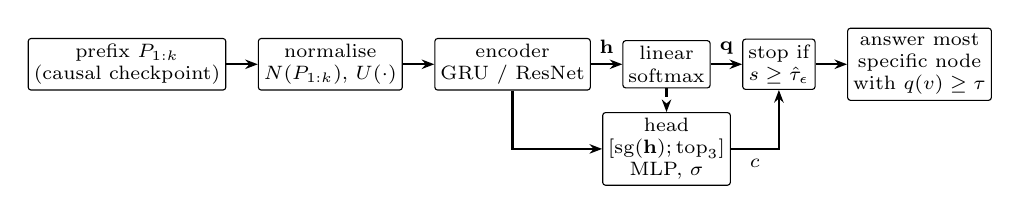
\begin{tikzpicture}[
  font=\scriptsize, node distance=3mm and 4mm,
  box/.style={draw, rounded corners=1pt, align=center, inner sep=2pt, minimum height=6mm},
  arr/.style={-{Stealth[length=1.6mm]}, thick}]
\node[box] (in) {prefix $P_{1:k}$\\(causal checkpoint)};
\node[box, right=of in] (norm) {normalise\\$N(P_{1:k})$, $U(\cdot)$};
\node[box, right=of norm] (enc) {encoder\\GRU / ResNet};
\node[box, right=of enc] (cls) {linear\\softmax};
\node[box, below=of cls] (head) {head\\$[\mathrm{sg}(\mathbf h);\mathrm{top}_3]$\\MLP, $\sigma$};
\node[box, right=of cls] (stop) {stop if\\$s \ge \hat\tau_\epsilon$};
\node[box, right=of stop] (tree) {answer most\\specific node\\with $q(v)\ge\tau$};
\draw[arr] (in) -- (norm);
\draw[arr] (norm) -- (enc);
\draw[arr] (enc) -- node[above] {$\mathbf h$} (cls);
\draw[arr] (enc) |- (head);
\draw[arr] (cls) -- node[above] {$\mathbf q$} (stop);
\draw[arr, dashed] (cls) -- (head);
\draw[arr] (head) -| node[pos=0.25, below] {$c$} (stop);
\draw[arr] (stop) -- (tree);
\end{tikzpicture}
\caption{The guesser at one checkpoint. The stopping score $s$ is the max softmax, the margin or
the head's confidence $c$; $\hat\tau_\epsilon$ is calibrated on validation data to bound the
accuracy gap (Sect.~\ref{sec:method-risk}). The tree answer (Sect.~\ref{sec:method-tree}) uses
its own threshold. Dashed: detached input.}
\label{fig:arch}
\end{figure}

\subsection{Stopping with a guaranteed accuracy gap}
\label{sec:method-risk}
A stopping rule should not lose much of what waiting would have won. Following Ringel et
al.~\cite{ringel2024early} (marginal version), the \emph{accuracy gap} of threshold $\tau$ is the
share of drawings whose final answer is right but whose early answer is wrong,
\begin{equation}
G(\tau) = \frac{1}{n}\sum_{i=1}^{n} \mathbf{1}\big[\hat y_{i,m} = y_i\big]\,
\mathbf{1}\big[\hat y_{i,j^\ast(\tau)} \ne y_i\big].
\end{equation}
On a calibration set of $n$ drawings we test thresholds from the highest to the lowest
(fixed-sequence testing, as in Learn then Test~\cite{angelopoulos2021ltt}) and keep going while the
one-sided Clopper--Pearson upper bound~\cite{clopper1934} of level $1-\delta$ on $G(\tau)$ stays at
most $\epsilon$; $\hat\tau_\epsilon$ is the last threshold accepted (answer at the end if none is).
Under exchangeability of calibration and test drawings, the population gap of $\hat\tau_\epsilon$
exceeds $\epsilon$ with probability at most $\delta$. We use $\delta = 0.05$ and
$\epsilon \in \{2\%, 5\%\}$. The guarantee concerns the population gap: the gap measured on a finite
test sample can exceed $\epsilon$ by sampling noise, and the guarantee does not cover a change of
distribution such as unseen countries.

\subsection{Coarse-to-fine answers on a class tree}
\label{sec:method-tree}
A tree groups the $C$ classes into subgroups and groups; a node $v$ covers a class set $S_v$ and
gets probability $q(v) = \sum_{c \in S_v} q_c$. At each checkpoint the hierarchical rule answers the
most specific node with $q(v) \ge \tau$ (smallest $|S_v|$, ties broken by probability) or stays
silent;
the flat rule answers the top class only when $q_c \ge \tau$. A correct answer earns
$r(v) = 1 - \log|S_v|/\log C$ (1 for a class, 0.76 for a 3-class subgroup, 0.34 for the 21-class
animal group), a wrong answer or silence earns 0~\cite{deng2012hedging}. The reward at a checkpoint
holds until the next one, giving a step function of ink, and the \emph{reward area} of a drawing is
\begin{equation}
R = \sum_{j=1}^{m} r_j\,(\ink_{k_{j+1}} - \ink_{k_j}), \qquad \ink_{k_{m+1}} := 1,
\end{equation}
averaged over drawings (higher means more correct information, earlier). For each tree and rule,
$\tau$ is the lowest value on a grid $\{0.30, 0.31, \dots, 0.99\}$ whose answers on the calibration
set are right at least 95\% (or 90\%) of the time. This choice uses a point estimate and has no
statistical guarantee, unlike Sect.~\ref{sec:method-risk}.

The \emph{semantic} tree (10 groups, 28 subgroups) follows everyday meaning, what a player would
say, and was frozen before any hierarchical result was computed. Two controls isolate what
matters: a \emph{random} tree with the same shape and shuffled classes (5 shuffles), and a
\emph{shape} tree with one level of clusters of early-drawing shape taken from the class-selection
analysis.

\section{Experimental Setup}
\label{sec:setup}

\subsection{Data}
\label{sec:setup-data}
\paragraph{Source and licence.} We use the \texttt{train\_simplified} files of the Kaggle
Quick, Draw! competition~\cite{kaggle_quickdraw}, drawn from Google's Quick, Draw!
dataset~\cite{quickdraw_dataset} (CC~BY~4.0). The drawings were collected by an online game in
which a player draws a given word within 20 seconds while a neural network tries to guess it; a
\texttt{recognized} flag records whether it did. The simplified version is aligned to the top-left
corner, scaled so that the longer side is 255, resampled at one-pixel spacing and simplified
with Ramer--Douglas--Peucker at $\epsilon = 2$~\cite{quickdraw_dataset}.

\paragraph{Subset.} We keep 100 of the 345 classes and 30{,}000 drawings per class (3{,}000{,}000
drawings). The classes were chosen from an analysis of early drawing shape: 76 are confusable
with another class early in the drawing, the others serve as controls; the selection and its
rationale are in the repository. Each drawing is a sequence of strokes: the median drawing has 4
strokes (p95 13, p99 19) and 41 points (p95 96, p99 151), and 15.6\% have a single stroke.

\paragraph{Quality.} No \texttt{key\_id} is repeated, but 39 groups of drawings have identical
strokes under different labels; we drop all 99 rows involved. 298 drawings have at most two points,
51 have no ink, and 0.85\% do not match the stated normalisation (offset above 2 or longer side
below 253). We keep them, since a game would see them too.

\paragraph{Biases.} 8.24\% of drawings were not recognised by the game, from 2.3\% for
\emph{triangle} to 18.5\% for \emph{bat}. Players come from 207 countries, but 44.3\% are from
the US and 69.9\% from the ten largest countries. The game stops a round once its model
recognises the drawing, so for the 91.8\% recognised drawings ``100\% ink'' means ``the round
stopped'', not ``the drawing was finished''. On the raw timed strokes of two classes, recognised
drawings were much shorter (median 1.9\,s for recognised triangles against 15.7\,s for the
others), and ink fraction correlated only 0.55 with elapsed time. Earliness in this paper is
therefore measured in ink, not in time.

\subsection{Splits and leakage prevention}
\label{sec:setup-splits}
The data is split per class into 24{,}000 / 3{,}000 / 3{,}000 drawings for training, validation and
test (seed 42), with identical drawings always in the same split (Table~\ref{tab:data}). Five
countries are held out entirely: IN, IT, KR, SA and TH, the largest country of five regions among
those with at least 100 drawings in every class, outside the ten largest. They were chosen from
counts and geography only, before any model was trained, and are removed from training,
validation and test at load time. No African or South American country met the rule.

% Generated by paper/make_assets.py from reports/preprocessing/split_summary.csv, reports/final_v1_*/results.json. Do not edit by hand.
\begin{table}[t]
\centering
\caption{Data after preprocessing (split v1, 100 classes). \emph{Used}: drawings left once the five
held-out countries are removed; those countries are scored separately (all their drawings, from all
three splits). Recog., US: share in \%. Strokes / points: medians.}
\label{tab:data}
\setlength{\tabcolsep}{4pt}
\begin{tabular}{lrrrrrc}
\toprule
Split & Drawings & Used & Recog. & US & Countries & Strokes / points \\
\midrule
train & 2{,}399{,}901 & -- & 91.8 & 44.3 & 207 & 4 / 41 \\
val & 300{,}000 & 281{,}492 & 91.8 & 44.2 & 185 & 4 / 41 \\
test & 300{,}000 & 281{,}291 & 91.7 & 44.2 & 191 & 4 / 41 \\
held out & -- & 185{,}544 & -- & 0.0 & 5 & -- \\
\bottomrule
\end{tabular}
\end{table}


Every decision (input normalisation, checkpoint, thresholds, trees, hyper-parameters) was taken
on validation data. For stopping and hierarchy experiments, validation is split once, per class,
into a \emph{calibration half} and an \emph{evaluation half} of 100 drawings each (seed 2026):
thresholds come from the first, reported numbers from the second. The data loader refuses to open
the test split or the held-out countries unless called by the final evaluation, which ran once,
after a gate that recomputed every validation number from the saved checkpoints and stopped on
any difference above 0.002 (86 numbers compared, largest difference 0.00195). The final
evaluation reuses the validation calibration half for thresholds; nothing is re-chosen on test.

\subsection{Training protocol}
\label{sec:setup-train}
All models are trained from scratch with AdamW~\cite{loshchilov2019adamw} (learning rate
$10^{-3}$, weight decay 0.01), 500 warm-up steps then cosine decay, batches of 512 prefixes,
gradient clipping at 1.0 and mixed precision, on a random subset of 600{,}000 training
drawings (6{,}000 per class, drawn with the run's seed). Each training example is a prefix with ink fraction uniform in
$[0.05, 1]$, after a random affine augmentation applied before normalisation (rotation
$\pm10^\circ$, independent axis scaling in $[0.9, 1.1]$, shear 0.1, no flips, since symmetry was
not checked per class). Baselines train for 8 epochs of one prefix per drawing; the method trains
for 4 epochs of two prefixes per drawing, so both take the same 9{,}375 steps of 512 prefixes. A
second pair trains both for twice as many steps (16 epochs of one prefix, 8 epochs of two). After
every epoch, the checkpoint is scored by its mean top-1 over ink fractions
$\{0.1, 0.25, 0.5, 0.75, 1\}$ on 200 validation drawings per class, and the best is kept. Every
condition is trained with seeds 42 and 43, except the $2\times$ runs (seed 42 only). Runs used
Kaggle notebooks with two NVIDIA T4 GPUs, PyTorch 2.11 and Python 3.13.

\subsection{Metrics}
\label{sec:setup-metrics}
\paragraph{Leak (H1).} Top-1 accuracy at ink fractions 10, 25, 50, 75 and 100\%, and \emph{early
top-1}, its mean over 10, 25 and 50\%, on 1{,}000 validation drawings per class and on every test
drawing. Top-3, macro-F1 and calibration error are recorded as well.
\paragraph{When to guess (H2).} The AUC of Sect.~3.1 is primary. It summarises all thresholds, but
it uses mean earliness, it rewards a frontier point regardless of whether a threshold could be
chosen to reach it, and its frontier is taken on the evaluation drawings, which flatters every
method equally. We therefore also report the risk-controlled operating points (realised gap,
accuracy and earliness at $\epsilon = 2\%$ and $5\%$), which do choose the threshold in advance.
\paragraph{Hierarchy (H3).} Reward area at precision 0.95 (primary) and 0.90, with the realised
precision and the share of checkpoints answered. The reward measures information, not usefulness
to a player, and depends on the tree's sizes.

\subsection{Baselines and experiments}
\label{sec:setup-matrix}
Table~\ref{tab:matrix} lists the trained conditions. The stopping baselines are the maximum
softmax probability~\cite{hendrycks2017baseline} and the margin of a standard classifier, a rule
that answers after a fixed number of strokes, and an oracle that answers at the first correct
checkpoint (unreachable, for reference). The hierarchy baseline is the flat rule with its own
calibrated threshold. As an off-the-shelf base model for the raster input, we fine-tune
torchvision's ResNet-18~\cite{he2016resnet} from its ImageNet weights, unchanged apart from its last
layer (the grey image is repeated over three channels and normalised with the ImageNet statistics),
and train the same network from scratch to separate the effect of pretraining from that of size
(11.2M parameters against 2.8M). Both follow exactly the protocol of our CNN. They were added after
the test evaluation and therefore have validation results only (Sect.~\ref{sec:res-base}).

\begin{table}[t]
\centering
\caption{Trained conditions. All use 600{,}000 training drawings and seeds 42 and 43 unless
noted. Method: confidence head, consistency loss ($\lambda = 0.5$) and two prefixes per drawing.}
\label{tab:matrix}
\setlength{\tabcolsep}{3pt}
\begin{tabular}{p{2.2cm}p{1.3cm}p{2.3cm}p{5.4cm}}
\toprule
Experiment & Model & Input & Training \\
\midrule
Leak (H1) & GRU, CNN & full\_bbox & baseline, 8 epochs \\
& GRU, CNN & prefix & baseline, 8 epochs \\
& GRU & resampled, end points kept & baseline, 8 epochs \\
& GRU & uniform & baseline, 8 epochs \\
\midrule
When to guess (H2) & GRU, CNN & prefix & method, 4 epochs $\times$ 2 prefixes \\
& GRU & prefix, uniform & 2 prefixes and head, no consistency \\
& GRU & uniform & method, 4 epochs $\times$ 2 prefixes \\
& GRU & uniform & baseline 16 epochs; method 8 $\times$ 2 (seed 42) \\
& GRU & prefix & method 8 $\times$ 2, exploratory, not compute-matched (seed 42) \\
\midrule
Hierarchy (H3) & \multicolumn{3}{p{9.4cm}}{no training: saved predictions of the baselines, four trees} \\
\midrule
Base model & ResNet-18 (torchvision) & prefix & ImageNet weights or from scratch, 8 epochs; validation only \\
\bottomrule
\end{tabular}
\end{table}

\section{Results and Analysis}
\label{sec:results}

Validation numbers decided every step; the test numbers below come from the single final
evaluation. Where both are given, they agree within 0.2 points of top-1 and 0.003 of AUC.

\subsection{The scale leak (H1)}
\label{sec:res-leak}

\IfFileExists{figures/fig_prefix_example.pdf}{%
\begin{figure}[t]
\centering
\includegraphics[width=\linewidth]{fig_prefix_example}
\caption{One validation drawing and the three inputs for its first 25\% of ink. Dots are the
model's input points. In the full frame the prefix is visibly small; after rescaling by its own
box, the gaps between stored points reveal the magnification; uniform resampling evens them out.}
\label{fig:prefix}
\end{figure}}{}

% Generated by paper/make_assets.py from reports/final_v1_test, reports/leak_v1, reports/followup_v1. Do not edit by hand.
\begin{table}[t]
\centering
\caption{Claim 1, the scale leak. Top-1 accuracy (\%) at each ink fraction on the test split
(every test drawing, mean of seeds 42 and 43). Early: mean over 10, 25 and 50\% ink. $\Delta$: early
top-1 minus the same model with \emph{prefix} input, in points. The last column is the same early
top-1 on validation (1{,}000 drawings per class), where every decision was taken.}
\label{tab:leak}
\setlength{\tabcolsep}{3.5pt}
\begin{tabular}{llrrrrrrrr}
\toprule
& & \multicolumn{5}{c}{Top-1 at ink fraction (test)} & \multicolumn{2}{c}{Early (test)} & Early \\
\cmidrule(lr){3-7}\cmidrule(lr){8-9}
Model & Input & 10\% & 25\% & 50\% & 75\% & 100\% & top-1 & $\Delta$ & (val) \\
\midrule
GRU & prefix & 10.1 & 28.0 & 55.0 & 73.9 & 79.0 & 31.0 & -- & 31.2 \\
GRU & full\_bbox (leaky) & 23.6 & 41.5 & 62.2 & 76.0 & 80.0 & 42.4 & $+11.4$ & 42.5 \\
GRU & uniform & 8.6 & 26.5 & 54.4 & 73.4 & 78.3 & 29.8 & $-1.2$ & 29.9 \\
\midrule
CNN & prefix & 8.3 & 28.6 & 58.9 & 78.4 & 83.9 & 31.9 & -- & 32.0 \\
CNN & full\_bbox (leaky) & 23.4 & 44.1 & 66.7 & 80.5 & 84.8 & 44.7 & $+12.8$ & 44.8 \\
\bottomrule
\end{tabular}
\end{table}


\begin{figure}[t]
\centering
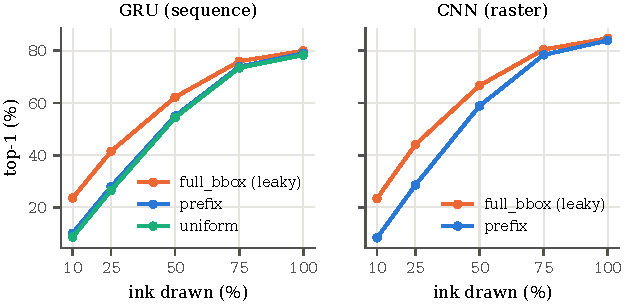
\includegraphics[width=\linewidth]{fig_leak}
\caption{Test top-1 against ink drawn (every test drawing, mean of two seeds). The leaky
full-frame input gains most when little is drawn; at 100\% ink all inputs see the same drawing.}
\label{fig:leak}
\end{figure}

Table~\ref{tab:leak} and Fig.~\ref{fig:leak} confirm the first part of H1. Keeping the finished
drawing's frame raises early top-1 by 11.4 points for the GRU and 12.8 points for the CNN on test,
and at 10\% ink it raises top-1 from 10.1\% to 23.6\% (GRU) and from 8.3\% to 23.4\% (CNN). The gain shrinks as
ink grows, as it should: at 100\% ink the two inputs are identical, and the remaining
0.9--1.0-point difference comes from training on different inputs. A model evaluated with the
finished drawing's frame would thus overstate early recognition several times over.

The second part, a residual leak in per-prefix inputs, took two attempts. Our pre-registered fix
resampled each stroke at even spacing but kept its end points; it cost 1.4 points of early top-1
on validation, more than the one-point margin we had set, so the rule kept \emph{prefix} input.
A separate audit then attacked the inputs directly. Reading the coordinate lattice of a rescaled
prefix recovers its size relative to the finished drawing within 3\% for 90.2\% of validation
prefixes, against 33.7\% for always guessing ``full size'' and 87.4\% on prefixes below 0.9 of the
full size. Using only stroke end points, which the first fix kept, still recovers it for 48.6\%.
After uniform resampling (Sect.~\ref{sec:method-norm}) the attack succeeds for 0.01\%. Regressors
trained to predict the log size ratio (gradient boosting on sequence features, a small CNN on
$64\times64$ rasters) reach $R^2 = 0.754$ on stored prefixes, 0.529 after uniform resampling and
0.501 on rasters. Part of this is legitimate, since shape alone says something about size: on two
classes for which we cut prefixes from the raw strokes and only then simplified them, the clean
inputs reach $R^2 \approx 0.55$. Against these clean references, stored sequences exceed by 0.24,
resampled sequences by 0.10 and rasters by 0.08. We therefore
report the GRU's early numbers with uniform input. It loses 1.2 points of early top-1 to
\emph{prefix} input on test (29.8 against 31.0) and 0.005 of stopping AUC on validation. This is an
upper bound on what the residual leak was worth to the GRU, because resampling also cuts corners
(raster IoU before and after: median 0.87). It is roughly ten times smaller than the full-frame
effect. For the CNN the residual is not measured in accuracy (Sect.~\ref{sec:limits}).

\subsection{When to guess (H2)}
\label{sec:res-anytime}

% Generated by paper/make_assets.py from reports/followup_v2_anytime, reports/anytime_v1_two_seeds. Do not edit by hand.
\begin{table}[t]
\centering
\caption{Claim 2a on validation (evaluation half, 100 drawings per class): area under the
accuracy--earliness frontier (AUC, higher is better) of the stopping policy named first (A) and
second (B). Upper block: GRU with uniform resampling, the leak-free sequence setting. $^\dagger$One
seed. Seed-to-seed range of a condition is at most 0.0026.}
\label{tab:ablation}
\setlength{\tabcolsep}{4pt}
\begin{tabular}{p{5.6cm}rrrc}
\toprule
Comparison (A vs B) & AUC A & AUC B & A $-$ B & Seeds \\
\midrule
Full method (head + consistency + 2 prefixes) vs baseline & 0.4467 & 0.4594 & $-0.0126$ & 2 \\
Confidence head vs max softmax, same classifier & 0.4467 & 0.4471 & $-0.0004$ & 2 \\
With vs without consistency loss & 0.4467 & 0.4521 & $-0.0054$ & 2 \\
Two prefixes per drawing alone vs baseline & 0.4523 & 0.4594 & $-0.0071$ & 2 \\
Margin vs max softmax (baseline model) & 0.4598 & 0.4594 & $+0.0004$ & 2 \\
$2\times$ steps, same compute: method vs baseline$^\dagger$ & 0.4746 & 0.4838 & $-0.0092$ & 1 \\
Baseline $2\times$ vs $1\times$ steps$^\dagger$ & 0.4838 & 0.4594 & $+0.0244$ & 1 \\
\midrule
GRU, prefix input: method vs baseline & 0.4548 & 0.4648 & $-0.0099$ & 2 \\
\midrule
CNN: method vs baseline & 0.4938 & 0.4999 & $-0.0061$ & 2 \\
\bottomrule
\end{tabular}
\end{table}

% Generated by paper/make_assets.py from reports/final_v1_test/results.json. Do not edit by hand.
\begin{table}[t]
\centering
\caption{Claims 2a and 2b on the test split (500 drawings per class, 50{,}000 drawings), thresholds
from the validation calibration half. AUC and end accuracy (\%, answer at the end of the drawing):
mean of two seeds. Risk control with target gap $\epsilon$: worst realised gap over the two seeds
(\%), then mean accuracy (\%) and mean ink used when answering. $^\ast$Realised gap above
$\epsilon$ for one seed. Over every run, stopping score and target, 38 of 40 are met.}
\label{tab:test_anytime}
\setlength{\tabcolsep}{2.6pt}
\begin{tabular}{lllrrrrrrrr}
\toprule
& & & & End & \multicolumn{3}{c}{$\epsilon = 2\%$} & \multicolumn{3}{c}{$\epsilon = 5\%$} \\
\cmidrule(lr){6-8}\cmidrule(lr){9-11}
Model & Training & Stopping score & AUC & acc. & gap & acc. & ink & gap & acc. & ink \\
\midrule
GRU & baseline & max softmax & 0.458 & 78.5 & 1.93 & 77.2 & 0.839 & 4.85 & 75.1 & 0.766 \\
GRU & baseline & margin & 0.458 & 78.5 & 1.90 & 77.2 & 0.840 & 5.04$^\ast$ & 74.9 & 0.765 \\
GRU & method & head & 0.446 & 75.6 & 1.86 & 74.6 & 0.838 & 4.46 & 72.7 & 0.770 \\
GRU & method & max softmax & 0.447 & 75.6 & 1.91 & 74.6 & 0.842 & 4.44 & 72.7 & 0.771 \\
\midrule
CNN & baseline & max softmax & 0.498 & 84.0 & 1.79 & 83.1 & 0.808 & 4.72 & 81.0 & 0.742 \\
CNN & baseline & margin & 0.497 & 84.0 & 1.84 & 83.1 & 0.806 & 4.45 & 81.1 & 0.744 \\
CNN & method & head & 0.491 & 82.5 & 1.94 & 81.6 & 0.810 & 4.76 & 79.6 & 0.743 \\
CNN & method & max softmax & 0.491 & 82.5 & 1.80 & 81.6 & 0.809 & 4.75 & 79.5 & 0.741 \\
\bottomrule
\end{tabular}
\end{table}


H2 is rejected. At equal compute, the method's stopping AUC is lower than that of the max-softmax
baseline in every comparison: by 0.013 for the uniform GRU on validation and 0.012 on test
(0.446 against 0.458), by 0.006 and 0.007 for the CNN (test 0.491 against 0.498), and by 0.010 for
the GRU with prefix input (Tables~\ref{tab:ablation} and~\ref{tab:test_anytime}). Seed-to-seed
ranges are below 0.003, so the sign is not in doubt. The learned confidence adds nothing over the
max softmax of the same classifier ($-0.0004$ on validation, $-0.0003$ on test): the head
recovers, at best, what the softmax already knows. The margin is equally close to the max
softmax ($+0.0004$), and a rule that answers after a fixed number of strokes is far behind (AUC
0.288 against 0.459 for the uniform GRU).

The ablations place the loss in the classifier, not the stopping score. Training on two prefixes
per drawing, with the head but without consistency, costs 0.007; adding the consistency loss
costs another 0.005. At a fixed number of steps, two prefixes per drawing means each drawing is
visited four times instead of eight, and the baseline is clearly under-trained: doubling its steps
adds 0.024 AUC and raises its end accuracy from 78.6\% to 81.6\%. An exploratory run that trained
the method twice as long (prefix input) had beaten the 1$\times$ baseline by 0.011, but its own max
softmax did the same (+0.011): the gain came from longer training. With both sides doubled, the
method still loses by 0.009 ($-0.008$ for its own max softmax).

\begin{figure}[t]
\centering
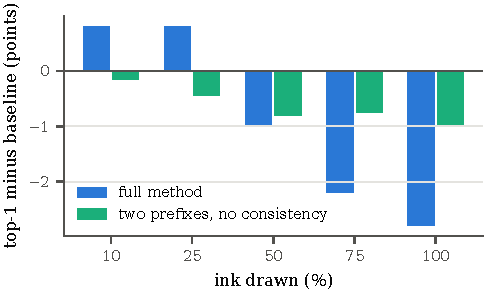
\includegraphics[width=0.75\linewidth]{fig_early_late}
\caption{Validation top-1 of the method and of two-prefix training without consistency, minus the
uniform-GRU baseline, at each ink fraction (two seeds). Consistency buys early accuracy with late
accuracy.}
\label{fig:earlylate}
\end{figure}

Fig.~\ref{fig:earlylate} shows what the consistency loss does. It improves top-1 by 0.8 points at
10\% and 25\% ink (9.6\% against 8.8\% at 10\%) and lowers it by 1.0 to 2.8 points from 50\% ink
on (75.7\% against 78.5\% at the end). Two prefixes without consistency are slightly worse at
every fraction. Pulling the short prefix toward the long one does make early predictions better,
as intended, but most accuracy, and hence most of the AUC, is earned after half the ink. We do not
know why late accuracy drops; two explanations we have \emph{not} tested are that the shared
encoder trades capacity toward short prefixes, and that a teacher which is itself often wrong at
mid-drawing propagates its errors.

\begin{figure}[t]
\centering
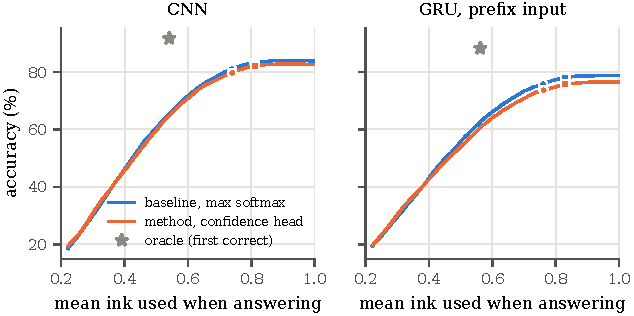
\includegraphics[width=\linewidth]{fig_frontier}
\caption{Accuracy against mean ink used, as the stopping threshold varies (validation evaluation
half, seed 42, prefix input; these are the runs whose full curves were saved). Squares and
circles: thresholds calibrated for $\epsilon = 2\%$ and $5\%$. Star: an oracle answering at the
first correct checkpoint.}
\label{fig:frontier}
\end{figure}

Fig.~\ref{fig:frontier} shows the size of the problem that remains. An oracle that answers at the
first correct checkpoint would be right 88--92\% of the time after 54--57\% of the ink, while the
calibrated threshold rules need 74--84\% of the ink to come within 2--5 points of their final
accuracy.
Neither score identifies the moment an answer becomes right.

\subsection{Stopping with a guaranteed accuracy gap}
\label{sec:res-risk}
Thresholds calibrated on 10{,}000 validation drawings kept the realised accuracy gap below its
target in 38 of 40 test cases (8 runs, 2--3 scores, 2 targets; Table~\ref{tab:test_anytime}). Both
misses use the margin score and exceed the target by little: 2.02\% for $\epsilon = 2\%$ and 5.04\%
for $\epsilon = 5\%$. With 50{,}000 test drawings, the standard error of a 5\% rate is about 0.1
point, so these are within sampling noise of a population gap at the target, which is what the
guarantee bounds. At $\epsilon = 5\%$, max-softmax stopping answers after 74\% of the ink for the
CNN (accuracy 81.0\% against 84.0\% at the end) and 77\% for the GRU (75.1\% against 78.5\%); at
$\epsilon = 2\%$ it needs 81--84\%. The guarantee holds, but the savings are modest: about a
quarter of the ink at a 5\% gap.

\subsection{Coarse-to-fine answers (H3)}
\label{sec:res-hier}

% Generated by paper/make_assets.py from reports/final_v1_test/results.json. Do not edit by hand.
\begin{table}[t]
\centering
\caption{Claim 3, hierarchical answers. Reward area (higher is better) of the answering rule with
each tree, at a precision target chosen on the validation calibration half; mean of two seeds.
Random: the semantic tree's shape with shuffled classes (5 shuffles). Shape: one level of
early-shape clusters. Gain: semantic minus flat. Prec.: realised precision of the semantic rule.}
\label{tab:hierarchy}
\setlength{\tabcolsep}{4pt}
\begin{tabular}{llrrrrrr}
\toprule
Target & Model & semantic & flat & random & shape & Gain & Prec. \\
\midrule
\multicolumn{8}{l}{\emph{Test split}} \\
0.95 & GRU uniform & 0.175 & 0.137 & 0.135 & 0.165 & $+0.038$ & 0.952 \\
0.95 & CNN prefix & 0.234 & 0.190 & 0.193 & 0.228 & $+0.043$ & 0.955 \\
0.90 & GRU uniform & 0.230 & 0.193 & 0.193 & 0.230 & $+0.038$ & 0.904 \\
0.90 & CNN prefix & 0.291 & 0.253 & 0.255 & 0.293 & $+0.038$ & 0.906 \\
\midrule
\multicolumn{8}{l}{\emph{Unseen countries}} \\
0.95 & GRU uniform & 0.172 & 0.132 & 0.131 & 0.159 & $+0.040$ & 0.942 \\
0.95 & CNN prefix & 0.233 & 0.189 & 0.192 & 0.225 & $+0.044$ & 0.943 \\
0.90 & GRU uniform & 0.226 & 0.188 & 0.188 & 0.222 & $+0.038$ & 0.887 \\
0.90 & CNN prefix & 0.289 & 0.250 & 0.252 & 0.288 & $+0.039$ & 0.889 \\
\bottomrule
\end{tabular}
\end{table}


H3 is confirmed (Table~\ref{tab:hierarchy}). At precision 0.95, the semantic tree raises the
reward area from 0.137 to 0.175 for the GRU and from 0.190 to 0.234 for the CNN on test, with
realised precision 0.952--0.956. It answers at 35\% of checkpoints against 23\% for flat answers
(GRU). A tree of the same shape with shuffled classes does no better than flat answers (0.135), so
the gain comes from which classes are grouped, not from having coarse nodes. The shape tree,
however, comes close: 0.165 at precision 0.95, a tie at 0.90 for the GRU (0.2297 against 0.2302), and
slightly ahead at 0.90 for the CNN (0.293 against 0.291). An
everyday-meaning tree is thus a good tree, but we cannot claim it beats one derived from how
drawings start.

\begin{figure}[t]
\centering
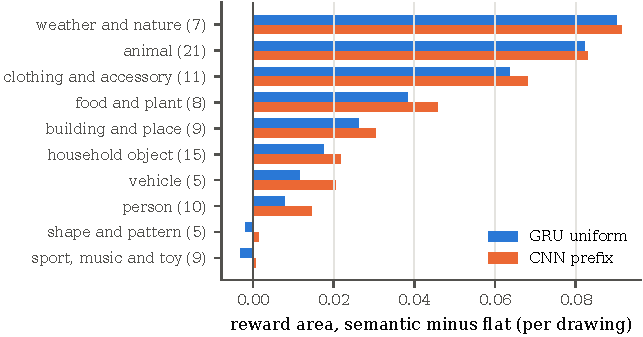
\includegraphics[width=0.75\linewidth]{fig_groups}
\caption{Gain of the semantic tree over flat answers per top-level group (validation evaluation
half, precision 0.95, mean of two seeds; number of classes in brackets).}
\label{fig:groups}
\end{figure}

Fig.~\ref{fig:groups} locates the gain. Weather and nature (+0.09 per drawing), animal (+0.08) and
clothing (+0.06) dominate; the 21 animal classes alone bring 40--44\% of the total gain. Shape and
pattern, and sport, music and toy gain nothing. The classes that gain most are tornado, hurricane,
sweater, jacket, horse, zebra and t-shirt, pairs whose early strokes look alike (spirals, garment
outlines, four-legged bodies) and also share a meaning. Where meaning and early shape coincide, a
group can be named long before the class; where they do not (a cello and a megaphone, a square and
camouflage), the group is no easier than the class. This also explains why the shape tree ties.

\subsection{Recognised and unrecognised drawings}
\label{sec:res-recognized}

% Generated by paper/make_assets.py from reports/analysis_v1/results.json. Do not edit by hand.
\begin{table}[t]
\centering
\caption{Validation AUC differences (A $-$ B) split by the game's \texttt{recognized} flag
(91.9\% of validation drawings are recognized).
Thresholds always come from the whole calibration half; only the evaluation half is split. End
accuracy of the runs analysed: 79.8--88.0\% on recognized
drawings, 27.3--36.3\% on unrecognized ones.
$^\dagger$One seed.}
\label{tab:recognized}
\setlength{\tabcolsep}{4pt}
\begin{tabular}{p{5.2cm}rrr}
\toprule
Comparison (A vs B) & All & Recog. & Unrecog. \\
\midrule
Method vs baseline, GRU uniform & $-0.0126$ & $-0.0121$ & $-0.0139$ \\
Same as above, $2\times$ steps$^\dagger$ & $-0.0092$ & $-0.0088$ & $-0.0097$ \\
Method vs baseline, GRU prefix & $-0.0099$ & $-0.0097$ & $-0.0123$ \\
Method vs baseline, CNN & $-0.0061$ & $-0.0056$ & $-0.0106$ \\
Uniform vs prefix input, GRU (max softmax) & $-0.0054$ & $-0.0071$ & $+0.0054$ \\
\bottomrule
\end{tabular}
\end{table}


Since a recognised drawing stops when the game recognised it, we repeat every comparison on the
two groups (Table~\ref{tab:recognized}). Every method-versus-baseline difference keeps its sign
in both. Unrecognised drawings are a different regime: end accuracy falls to 30--36\% and AUC to
about 0.2. There the uniform input is slightly \emph{better} than prefix input ($+0.005$
against $-0.007$ on recognised drawings); one reading, not tested further, is that the residual
leak helps mainly on recognised drawings.

\subsection{Unseen countries}
\label{sec:res-unseen}

% Generated by paper/make_assets.py from reports/final_v1_test/results.json. Do not edit by hand.
\begin{table}[t]
\centering
\caption{Held-out countries (IN, IT, KR, SA, TH; never seen in training or validation) against the
in-distribution test split. Top-1 (\%) at 10, 50 and 100\% ink on every drawing; AUC and worst
realised gap (\%) at $\epsilon = 5\%$ of max-softmax stopping on 500 drawings per class; mean of two seeds.}
\label{tab:unseen}
\setlength{\tabcolsep}{4pt}
\begin{tabular}{llrrrrr}
\toprule
Model & Set & 10\% & 50\% & 100\% & AUC & gap at 5\% \\
\midrule
GRU uniform & test & 8.6 & 54.4 & 78.3 & 0.458 & 4.85 \\
GRU uniform & unseen & 8.6 & 52.5 & 74.7 & 0.440 & 4.89 \\
\addlinespace
CNN prefix & test & 8.3 & 58.9 & 83.9 & 0.498 & 4.72 \\
CNN prefix & unseen & 8.3 & 57.2 & 80.8 & 0.484 & 4.71 \\
\bottomrule
\end{tabular}
\end{table}


On the five held-out countries (Table~\ref{tab:unseen}), end accuracy drops from 78.3\% to 74.7\%
(GRU) and from 83.9\% to 80.8\% (CNN), but early accuracy is unchanged (8.2--8.6\% at 10\% ink):
what differs between countries is the finished drawing, not its first strokes. Stopping AUC falls
by 0.014--0.019. Thresholds calibrated on validation still met the accuracy-gap target in 15 of 16
cases (one margin miss at 5.06\%), although the guarantee does not formally cover this shift. The
semantic tree's gain over flat answers is the same as in distribution (+0.040 GRU, +0.044 CNN),
but its realised precision falls to 0.941--0.944 for a 0.95 target.

\subsection{An off-the-shelf base model}
\label{sec:res-base}

% Generated by paper/make_assets.py from reports/pretrained_v1*, reports/hierarchy_pretrained_v1, reports/leak_v1. Do not edit by hand.
\begin{table}[t]
\centering
\caption{Off-the-shelf base model, \textbf{validation only} (added after the test split was opened).
Top-1 (\%) at 10 and 100\% ink and early top-1 (10--50\%) on 1{,}000 drawings per class; end accuracy (\%),
AUC and ink used at $\epsilon = 5\%$ of max-softmax stopping, and (Tree) semantic-minus-flat reward area at
precision 0.95, on the evaluation half. Project CNN: the \emph{cnn\_prefix} runs; ResNet-18:
torchvision's network. Mean of two seeds; same training protocol for every row.
$^\ast$Gap target missed for a seed.}
\label{tab:pretrained}
\setlength{\tabcolsep}{3pt}
\begin{tabular}{lrrrrrrrr}
\toprule
Model & Params & 10\% & 100\% & Early & End & AUC & Ink & Tree \\
\midrule
Project CNN & 2.8M & 8.4 & 83.9 & 32.0 & 83.8 & 0.500 & 0.740 & $+0.044$ \\
ResNet-18, scratch & 11.2M & 8.5 & 83.8 & 32.1 & 84.0 & 0.503 & 0.735 & $+0.041$ \\
ResNet-18, ImageNet & 11.2M & 9.0 & 85.0 & 33.1 & 84.9 & 0.512 & 0.723 & $+0.045$ \\
\bottomrule
\end{tabular}
\end{table}


To check that the conclusions do not rest on a small network of our own, we repeated the stopping
and hierarchy evaluations with torchvision's ResNet-18 (Table~\ref{tab:pretrained}, validation only).
Trained from scratch, it matches our CNN (top-1 83.8\% against 83.9\% at the end of the drawing, AUC
0.503 against 0.500) with four times the parameters, so our CNN is not a weak baseline for this
input. ImageNet weights help modestly: +1.1 points of top-1 at the end (85.0\%), +1.2 points of early
top-1 (33.1\% against 32.0\%), and +0.012 AUC, of which +0.009 over the same network from scratch.
Pretraining on photographs thus transfers a little to doodles, but does not change the picture.
The findings on stopping and on the tree hold for the pretrained model (the leak and the learned
stopping method were not re-run with it): the margin is not better than the max softmax
($-0.0015$); the risk-control targets are met for both seeds, both scores and both targets, and at
$\epsilon = 5\%$ it answers after 72\% of the ink instead of 74\%; and the semantic tree gains
$+0.045$ over flat answers and $+0.043$ over a shuffled tree, but only $+0.011$ over the shape tree at
precision 0.95 and $-0.004$ at 0.90. These models were added after the single test evaluation, so
they have no test numbers; elsewhere validation and test agree within 0.003 AUC, but we have not
shown it here.

\subsection{Successes and failures}
\label{sec:res-examples}

\IfFileExists{figures/fig_qualitative.pdf}{%
\begin{figure}[t]
\centering
\includegraphics[width=\linewidth]{fig_qualitative}
\caption{Max-softmax stopping of the CNN at $\epsilon = 5\%$ on validation drawings. Black: ink
seen when answering (percentage in brackets); gray: the rest of the drawing. Top: early and right.
Bottom: early and wrong, although the end of the drawing is classified correctly.}
\label{fig:qualitative}
\end{figure}}{%
\begin{figure}[t]
\centering
\fbox{\parbox{0.9\linewidth}{\centering\vspace{1cm}Run \texttt{python paper/make\_assets.py
--val-predictions <folder>} with the processed dataset to draw this figure.\vspace{1cm}}}
\caption{Qualitative successes and failures (placeholder).}
\label{fig:qualitative}
\end{figure}}

Fig.~\ref{fig:qualitative} shows typical cases. % TODO(Kiet): describe the drawn examples once the figure exists.
The model answers early and correctly when the first strokes are already distinctive, and fails
early when the first strokes are shared with another class and the deciding detail comes last.

\subsection{What did not work}
\label{sec:res-failed}
For completeness: (i) resampling that kept stroke end points did not remove the leak;
(ii) the learned stopping method lost to max softmax on every architecture, input and budget we
tried; (iii) its one apparent success, the exploratory $2\times$ run, was explained by training
length; (iv) the semantic tree did not beat a shape-derived tree; (v) an early version of the
risk-control code compared thresholds in float32 during calibration and float64 during evaluation
(NumPy type promotion); we fixed it and rescored, and every reported number was unchanged.

\section{Limitations}
\label{sec:limits}

\paragraph{Scale of the study.} We use 100 classes and train on 6{,}000 drawings per class, about a
quarter of the training split, with two seeds. The baseline gains 0.024 AUC from twice the steps, so
all models are under-trained, and we have not shown that the negative result for H2 survives
training to convergence. Seed ranges are small next to the reported differences, but two seeds
give no interval over data resampling.

\paragraph{The leak is reduced, not removed.} Uniform resampling removes the lattice and point
density but not the simplification facets: on the two classes with a clean reference, resampled
sequences still predict the size ratio better than clean ones. The raster model keeps a similar
residual whose effect on accuracy we did not measure. The only complete fix is to cut prefixes
from the raw strokes and simplify them afterwards, which needs the raw files (about 53\,GiB for 99 of our 100
classes). The 1.2-point cost of resampling mixes leak removal with lost detail.

\paragraph{Ink is not time.} Earliness is measured in ink, which correlated only 0.55 with time on
the two classes we checked, and 100\% ink is where the game stopped, which for 91.8\% of drawings is
when Google's model recognised it. A guesser that is ``early'' in ink may not be early in a real
game.

\paragraph{Guarantees.} The accuracy-gap bound is marginal over drawings and assumes calibration
and test drawings are exchangeable. It says nothing about individual classes, and it does not cover
shifts such as new countries, where it held in 15 of 16 cases without a formal reason to. The
hierarchy's precision target is met only in estimate; under the country shift it fell to about
0.94.

\paragraph{Controls and evaluation.} The shape tree comes from a class-selection analysis whose
statistics may include drawings now in the validation split, so that control may be slightly
favoured. The checkpoint-selection subset (200 validation drawings per class) can overlap the
calibration and evaluation halves, which makes validation numbers slightly optimistic; the test
numbers are not affected. The AUC uses mean earliness and an envelope taken on the evaluation
drawings. Only five held-out countries were tested, none from Africa or South America. The
off-the-shelf ResNet-18 was added after the test evaluation and has validation results only.

\section{Conclusion}
\label{sec:conclusion}

Early recognition of sketches is easy to overstate. Truncating drawings that were normalised as
finished drawings hands the model their final size; with the finished frame, early top-1 was more
than ten points higher, and per-prefix rescaling still leaked enough to be visible in the
coordinates. Once inputs are made fair, learning when to guess was harder than we expected: a
ConfidNet-style head with a prefix-consistency loss did not beat the maximum softmax probability
at equal compute, because two-prefix training and consistency cost late accuracy, which is where
most accuracy is earned. Two simpler tools did work. Distribution-free calibration gives stopping
thresholds whose accuracy loss is bounded, and it held on test and largely on unseen countries.
Answering the most specific safe node of a class tree gives a player useful information earlier,
mostly for groups whose members also start alike.

For a deployed guesser we would therefore use the CNN with prefix input (test top-1 83.9\% at
the end of the drawing), max-softmax stopping with a calibrated threshold, and the semantic tree;
the uniform-input GRU is the sequence alternative with the least leak. An ImageNet-pretrained
ResNet-18 is about one point better on validation and would be the stronger choice once confirmed on
fresh test data. Future work should cut
prefixes from raw strokes to remove the leak entirely, measure earliness in time, train to
convergence before revisiting learned stopping, and control the gap per class.

\paragraph{Code, data and checkpoints.}
% TODO(Kiet): add the public repository URL and the checkpoint download link before submission.
Code, configuration files, every reported number (\texttt{reports/}) and the scripts that produce
this paper's tables and figures (\texttt{paper/make\_assets.py}) are in the project repository,
with instructions for downloading the data and the trained checkpoints.

\paragraph{Use of AI assistance.}
% TODO(team): adjust to what each member actually used.
The team used Claude (Anthropic), an AI assistant, to help write and review code, design
experiment configurations, run and monitor the Kaggle notebooks, check references and draft
parts of this report. All experiments were run on our accounts, every number was produced by
the code in the repository, and the team reviewed the text and is responsible for all claims.
No proprietary model is part of the proposed method.


\bibliographystyle{splncs04}
\bibliography{references}

\end{document}
